\subsection{Il dataset} \label{textc_data}
Il dataset utilizzato è stato messo a disposizione dagli sviluppatori di SparkNLP (John Snow Lab) per un workshop da loro svolto e reso disponibile sul loro profilo Github\footnote{Repository: \href{https://github.com/JohnSnowLabs/spark-nlp-workshop/tree/master/tutorials/Certification_Trainings/Public/data}{https://github.com/JohnSnowLabs/spark-nlp-workshop/}}. 

Il dataset è composto da due file: \textit{news\_category\_train.csv} con 120.000 esempi per l’addestramento e \textit{news\_category\_test.csv} con 7.600 esempi per il testing.
Ogni riga di entrambi i file è formata dai campi \textbf{description} e \textbf{category}. Il primo contiene il testo da classificare, il secondo indica di quale categoria fa parte il testo. Ogni testo appartiene esattamente ad una sola classe.
In totale, ci sono 4 categorie: \textit{Business}, \textit{Sci/Tech}, \textit{World}, \textit{Sports}.\\
\begin{figure}[hbt!]
    \centering
    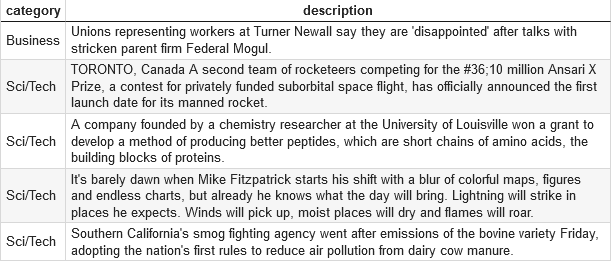
\includegraphics[width=0.9\textwidth]{img/textc_dataset.png}
    \caption{Porzione del dataset per Text Classification}
    \label{fig:textc_dataset}
\end{figure}